\documentclass{acmsiggraph}               % final

%% These two line bring in essential packages: ``mathptmx'' for Type 1
%% typefaces, and ``graphicx'' for inclusion of EPS figures.


\usepackage{graphicx}
\usepackage{url}
\usepackage{times}



%% Paper title.

\title{Simulate brushed metal surface in homegrown OpenGL render.}

%% Author / Affiliation (single author).

%%\author{Roy G. Biv}
%%\affiliation{Allied Widgets Research\thanks{email:roy.g.biv@aol.com}}

%% Author / Affiliation (multiple authors).

\author{Stefan Eng\thanks{e-mail: atn08sen@student.lth.se}
}
\affiliation{Lund University\\ Sweden}


%% Keywords that describe your work.
\keywords{OpenGL, from-scratch, brushed metal, C}

%%%%%% START OF THE PAPER %%%%%%

\begin{document}

\ifpdf
  \DeclareGraphicsExtensions{.jpg,.pdf,.mps,.png}
\else
  \DeclareGraphicsExtensions{.eps}
\fi


\maketitle

\begin{abstract}
The main motivation for the project is to get accustomed with the possibilities
and limitations of doing low level OpenGL programming from scratch in C. The projects
graphical focus is to simulate a brushed metal surface with semi-realistic light
reflections. \\

The final approach to the surface simulation includes a
tangent-map texture to simulate the topography texture of a brushed metal
in combination with a standard
Phong\footnote{\url{https://en.wikipedia.org/wiki/Phong_shading}} shading model to achieve the desired
result. Ideally this method would be compared to a more procedural approach in combination
with a slightly more advanced light model like the
Blinn-Phong\footnote{\url{https://en.wikipedia.org/wiki/Blinn–Phong_shading_model}} model. This was
never done due to the render backbone implementation hitting a few problems and
taking loger then anticipated.

\end{abstract}


\section{Introduction}

\begin{figure}[!ht]
    \centering
    
\includegraphics[width=0.7\columnwidth]{brushed.jpg}
    \caption{Photo of brushed metal.}
    \label{brushed_real}
\end{figure}

Brushed metal is a common type of metal texture on cookwares such as pots and
pans and can also be found on metallic counter tops. One of the more
recognizable properties of brushed metals is its ability to produce anisotropic
highlights.

\begin{figure}[!ht]
    \centering
    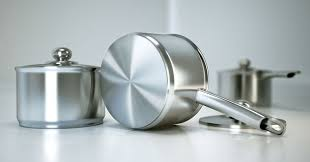
\includegraphics[width=0.7\columnwidth]{highlight.jpg}
    \caption{Example of anisotropic specular highlight.}
    \label{anisotropic_highlight}
\end{figure}

%As part of the course EDAN35, each group of two\footnote{In some cases, groups with only three or one student
%have to be formed, but this should be avoided as much as possible.} students need to create
%a project as well. The project should be a 3D Graphics applications based on a 3D engine, for example the framework used in the assignements.
%The project is worth 3 points.
%
%Any group who wants can participate in the competition.

\section{3D Graphics Project}
In this project, you have a lot of freedom. You need to write
an application using a 3D Graphics API, such as OpenGL, a rendering engine, such as the C++ framework used in the labs, which is either
cool, beautiful, interesting, useful, fun to use, or a combination of all of the above.
Examples of applications may include:
\begin{itemize}
    \item 3D graphics algorithm. From recent paper or GPU programming text, such as GPU Gems
    \item game
    \item screensaver
    \item 3D GUI for mobile platforms
    \item useful tool
    \item something completely different
\end{itemize}
Remember though that as a group of two, you need to spend nearly 6 weeks on this.
This obviously means that if you decide to make a screen saver, it should be \textit{very}
challenging, otherwise, you will not pass.

The performance of your application is not the most important thing for the project. If you do
optimize for performance, that is a good thing (especially for the competition).

You can use the code from the \textit{Deferred Shading Assigment} when you start with this type of project.

\subsection{Who wins the 3D Graphics competition?}
A jury will decide at the last lecture.

The deadline is at 13:00 on the day before the last lecture and competition.
The report and code should be delivered by then. However, note that modifications
to the code can be done after that (in order to further impress the jury).

\section{Written Report}

The report should be handed in an PDF format. You can use any word processing software you like, but you need to generate a PDF for the final submission.

The typesetting for this paper was done using pdf\LaTeX. It is recommended that you
use this as well, and therefore the ``source files'' for this very document are
available on the course website. If you are not familiar with pdf\LaTeX, then
you may use whatever other word processing program you like, as long as you mimic
the general style in this paper (i.e., you paper should look similar to
this paper).

The source files consists of two style files: \texttt{acmsiggraph.bst}
and \texttt{acmsiggraph.cls}, and these should be placed in the directory as the
files \texttt{project.tex} and \texttt{project.bib}. There is also a PNG image called
\texttt{lugg.png} that is shown later in this paper.
It is in \texttt{project.tex}, where you should delete this document's text,
and instead write your own text.

You should write your report as a scientific paper. It should have (at least)
the following sections:
\begin{itemize}
    \item Abstract [brief summary of key results]
    \item Introduction [why do what we did? motivation]
    \item Algorithms or Application [description of what you did, what algorithms you implemented]
    \item Results [e.g., performance, \textbf{screenshots}, usefulness etc]
    \item Discussion [what did not work, what worked well, what can be improved, optimizations you tried]
    \item Conclusion [any concluding remarks -- skip if you do not have anything to say in addition to what you've already said]
\end{itemize}
Some groups may not have enough important material to write a ``Discussion''-section,
and in such cases, that section can be omitted. Also, look at scientific papers,
e.g.,~\cite{Hakura97,Igehy98,RaganKelley2011,Doggett2012,Ganestam2015}, and try to follow their general style.
When in doubt, come and ask us.
If you need references not found in the file \texttt{project.bib}, simply add your reference to
that file. The report should be 2--4 pages long.

You can include screenshots as PNGs or illustrations in the PDF format.
An example is shown in Figure~\ref{fig_lugg}. See the source file \texttt{project.tex}
for how this is done in \LaTeX.
\begin{figure}[tb]
    \centering
    
\includegraphics[width=0.7\columnwidth]{lugg.png}
    \caption{This is the logotype for LUGG: Lund University Graphics Group.}
    \label{fig_lugg}
\end{figure}

\section{Conclusion}
Make a great project. You're clever. Surprise us (and the jury)!

\bibliographystyle{acmsiggraph}
%\nocite{*}
\bibliography{project}
\end{document}
